\bigskip

\item The graphs of $f$ and $g$ are shown in the figure below.  Estimate the value of $g(f(3))$.

% \resizebox{3in}{!}{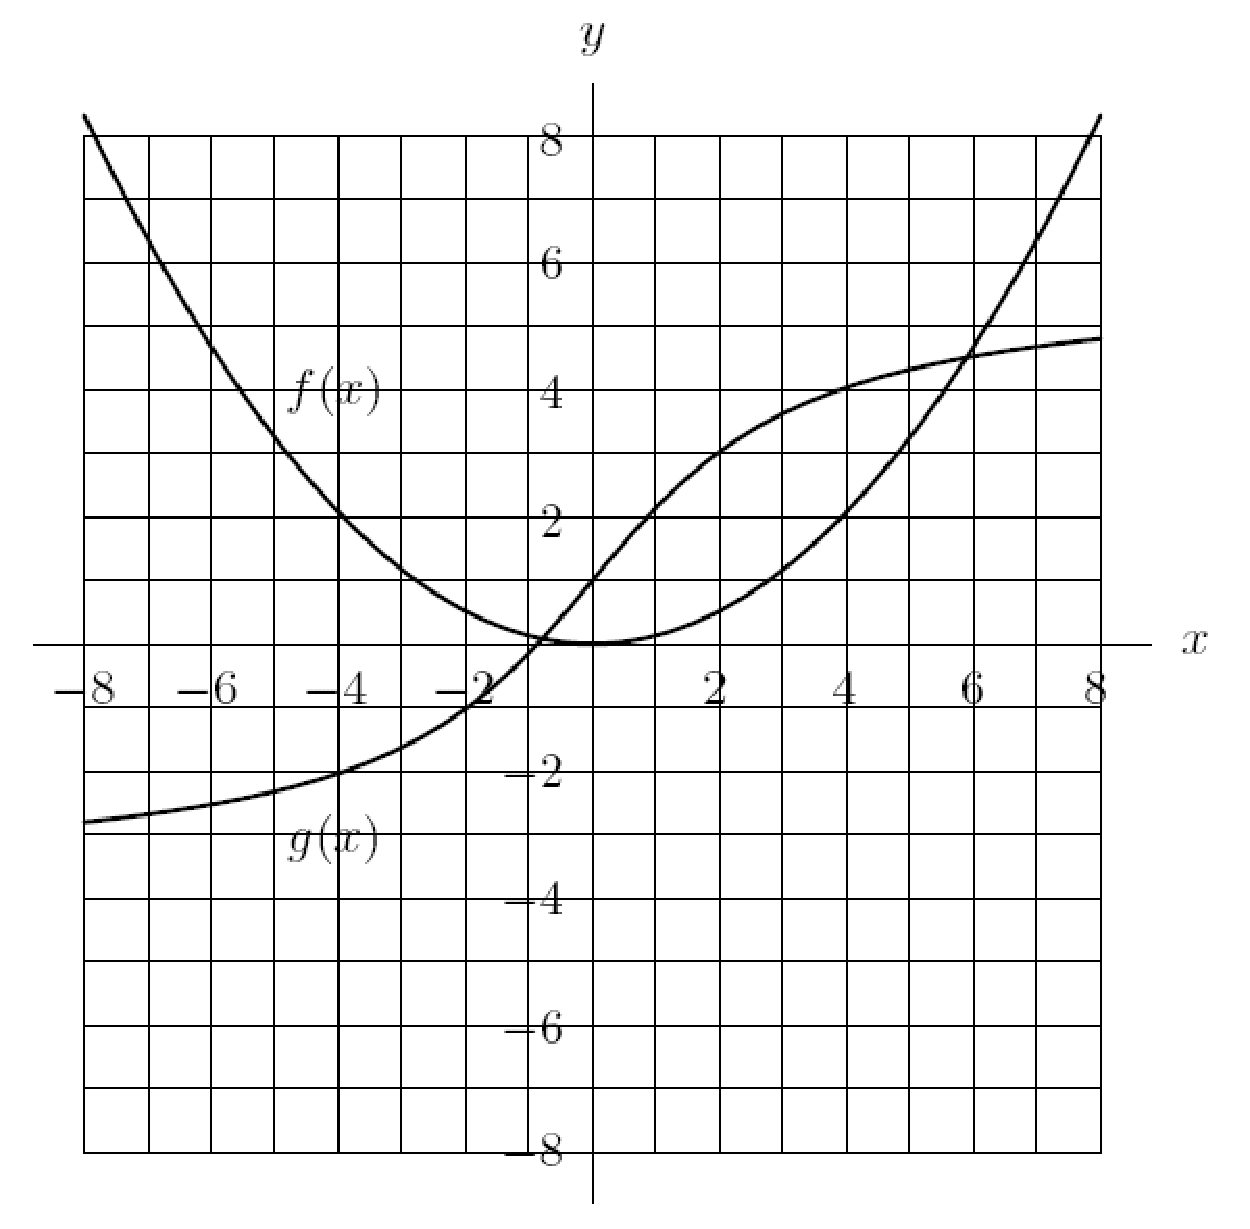
\includegraphics{SVC.01.03.030.ps}}

\begin{minipage}{0.3\columnwidth}
    \begin{enumerate}
        \item -1 
        \item 0
        \item 1
        \item 2
        \item 3
        \item 5
    \end{enumerate}
\end{minipage}
\begin{minipage}{0.7\columnwidth}
    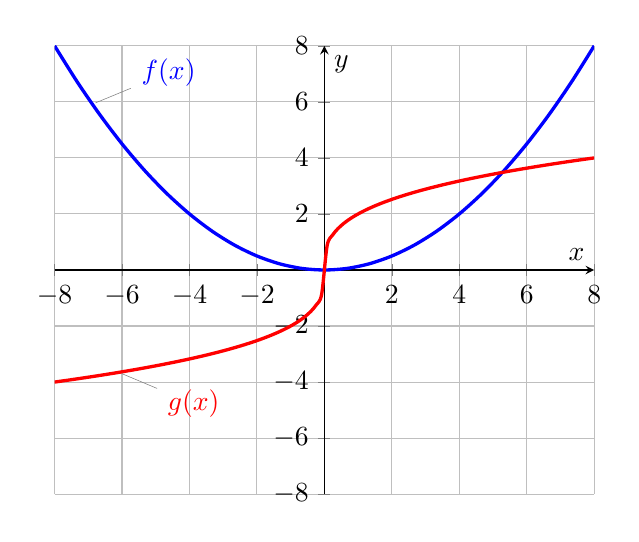
\begin{tikzpicture}
        \begin{axis}[axis lines=center, xlabel={$x$}, ylabel={$y$}, grid, xmin=-8, xmax=8,
            ymin=-8, ymax=8, xtick={-8,-6,-4,-2,2,4,6,8}, ytick={-8,-6,-4,-2,2,4,6,8}]
            \addplot[blue,very thick, smooth, domain=-8:8] {(1/8)*x^2} node[pos=.1,pin={10:$f(x)$}, inner sep=0pt] {};
            \addplot[red,very thick, smooth, domain=-8:8, samples=100]
            {2*x/abs(x) * (abs(x))^(1/3)} node[pos=.1,pin={-10:$g(x)$}, inner sep=0pt] {};
        \end{axis}
    \end{tikzpicture}
\end{minipage}

% ConcepTests - to accompany Calculus 4th Edition, Hughes-Hallet et al. John Wiley \& Sons.
